\section{Umsetzung des Prototypen emoTrix}
Hier werden Dinge umgesetzt.
\subsection{MockUps}
\subsection{Datenerfassung in Form von Emotionstests}
\subsubsection{GSR-Test}
\subsubsectionauthor{Lukas Seemann}
Die Erfassungsmöglichkeit mit der höchsten Priorität war die Messung der Hautleitfähigkeit mithilfe von EDA- beziehungsweise GSR-Sensoren. Da dies nicht mit im Smartphone enthaltenen Sensoren möglich war, wurde zusätzlich ein Arduino-Mikrocontroller benötigt, um die Messung durchzuführen. Zunächst wird die Entwicklung auf dem Arduino-Board mit allen zusätzlichen Modulen beschrieben. Im Anschluss daran wird thematisiert, wie das Arduino-Board mit der App verbunden wurde. \newline
Für das Projekt wurde ein Arduino UNO R3 Board verwendet. \footcite[Vgl.][]{Ard18} Dieser kann mit Stromzufuhr über ein Netzteil oder per USB betrieben werden. Als Sensor wurde ein GSR Sensor des Grove-Toolkits verwendet\footcite[Vgl.][]{Gro18}, der bereits in Abbildung 5 gezeigt wird. Am Sensor selbst werden die Elektroden für die Finger angebracht. Da ein handelsübliches Arduino UNO R3 Board nicht über den benötigten Anschluss für den Grove GSR-Sensor verfügt, muss zusätzlich noch ein Grove Base Shield angebracht werden. Dieses kann auf das Arduino Board aufgesteckt werden und erweitert es um viele verschiedene Anschlüsse, unter anderem für Sensoren.
\begin{figure}[h]
	\centering
	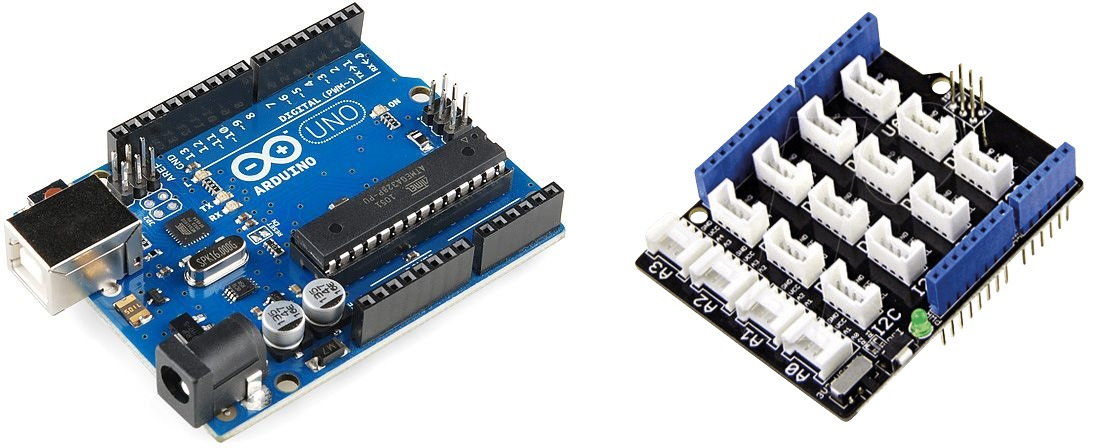
\includegraphics[width=16cm]{Bilder/arduino.jpg}
	\caption[Arduino UNO R3 (links) und Grove Base Shield]{Arduino UNO R3 (links) und Grove Base Shield\footnotemark}
\end{figure}%
\footcitetext[Bilder von:][]{Sou18, Rei18}
\newline 
Mit diesen Komponenten werden die vom Sensor zurückgelieferten Daten an den Arduino geleitet. Von dort aus müssen die Daten, an die mobile Applikation weitergeleitet werden. Aus diesem Grund muss an das Arduino Board ein Bluetooth-Modul angebracht werden, das Daten senden und empfangen kann. Das Empfangen von Daten ist notwendig, um die Messung zu Starten, wohingegen das Senden für die Übermittlung der Sensordaten benötigt wird. Heutige Smartphones verfügen meistens immer über eine Bluetooth-Schnittstelle, aus welchem Grund Bluetooth gut für die Übertragung geeignet ist. Eine weitere Möglichkeit wäre die Übertragung über WiFi gewesen. Das Arduino-Board wurde mit einem HC05-Bluetooth-Modul erweitert, welches Daten senden und empfangen kann. Dieses ist in Abbildung ? zu sehen.
\begin{figure}[h]
	\centering
	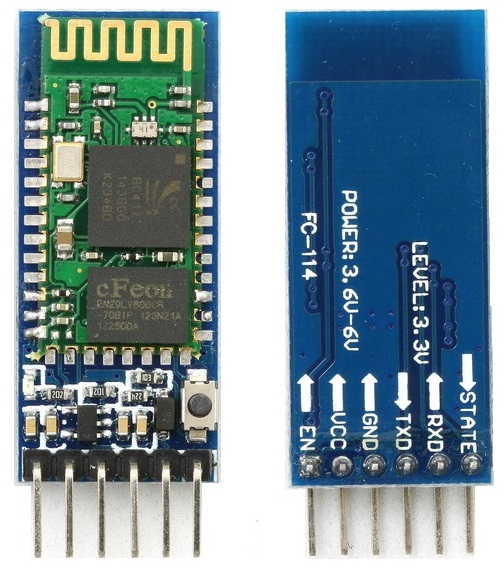
\includegraphics[width=6cm]{Bilder/hc05.jpg}
	\caption[HC-05-Bluetooth-Modul für Arduino]{HC-05-Bluetooth-Modul für Arduino\footnotemark}
\end{figure}%
\newline
Die Beschreibung der Entwicklungsarbeiten wird in zwei Teile aufgespalten. Der erste Teil ist der Quellcode des Arduinos, der zweite Teil die Entwicklung des Emotionstest in der emoTrix-App. \newline
In Listing ? ist der Quellcode des Arduinos abgebildet. In Zeile 1 wird die SofwareSerial-Bibliothek eingebunden, die eine Verwendung der Pins des Arduinos für verschiedene Module ermöglicht. In Zeile 2 wird dem Arduino mitgeteilt, dass auf den Pins 10 und 11 ein Bluetooth-Modul angeschlossen ist und eine Konstante (GSR) festgelegt, die auf den Anschluss A0 des Grove Shields verweist, an dem der GSR Sensor angeschlossen ist. \newline
Generell besteht der Programmcode des Arduinos immer aus zwei Bestandteilen: einem Setup-Block und einem Loop-Block. Der Setup-Block wird einmalig beim Einschalten des Arduinos ausgeführt. Danach wird der Loop-Block solange wiederholt, bis der Arduino ausgeschalten wird. \newpage

\begin{lstlisting}[caption={Quellcode des Arduinos},style=Arduino]
#include <SoftwareSerial.h>
SoftwareSerial BTserial (10, 11); const int GSR=A0;
int sensorValue=0; int gsr_average=0;
boolean measuring = false; char BTString;

void setup(){
	BTserial.begin(9600);
}

void loop(){
	BTString = BTserial.read();
	if(BTString == 'S'){
		measuring = true;
	}
	if(BTString == 'F'){
		measuring = false;
	}
	if(measuring){
		long sum=0;
		for(int i=0;i<10;i++){ 
			sensorValue=analogRead(GSR);
			sum += sensorValue; delay(5);
		}
		gsr_average = sum/10;
		BTserial.print(gsr_average); BTserial.println( ";");
	}
}
\end{lstlisting}
In Zeile 7 innerhalb des Setup-Blocks wird die Geschwindigkeit der seriellen Datenübertragung der Ports des Arduinos, die mit dem Bluetooth-Modul verbunden sind. Hierbei wird die Geschwindigkeit auf 9600 Bits pro Sekunde gesetzt.\footcite[Vgl.][]{Ard18b} Dies entspricht der üblich verwendeten Geschwindigkeit und hat in Tests sehr gut funktioniert. \newline
Der Loop-Block beginnt in Zeile 11 mit dem Auslesen der Daten, die über das Bluetooth-Modul empfangen werden. Die Variable \textit{BTSTring} wird mit diesen Daten beschrieben. Die App muss zum Starten der App den String \textit{S} (für Start) per Bluetooth übertragen. Ist dies der Fall, wird die Variable \textit{measuring} auf true gesetzt. Mit dem String \textit{F} (für Finished) kann die App dem Arduino das Stopsignal für die Messung geben. Demenstprechend wird \textit{measuring} auf false gesetzt. Dies ist in den Zeilen 15 bis 17 umgesetzt. \newline
In Zeile 18 wird über die \textit{measuring}-Variable überprüft, ob gemessen werden soll. Wenn ja, wird eine Variable für die Summe von 10 Messdaten initialisiert. Anschließend werden in Abstand von 5 Millisekunden 10 Messungen durchgeführt. In Zeile 21 wird die eigentliche Messung des Sensors durchgeführt. Der hier verwendete GSR-Sensor liefert die aktuell gemessene Stromspannung an der Haut als Integer-Wert zurück. Alle 10 Messungen werden nach und nach aufaddiert. Dies geschieht in der for-Schleife in den Zeilen 20 bis 23. Anschließend wird die Summe durch 10 geteilt, sodass man den Durchschnitt aller 10 Werte erhält. Dieses Verfahren wird durchgeführt, da die Messdaten des Sensors Schwankungen aufweisen, die dadurch eliminiert werden können. In Zeile 25 wird schließlich der Messwert auf den Port des Bluetooth-Moduls geschickt und damit versendet. Als Trennzeichen zum nächsten Wert wird ein Semikolon angehängt. \newline
Wenn die Messung gestartet wurde, erhält die mobile Applikation  also alle 50 Millisekunden vom Arduino per Bluetooth einen Integer-Wert, der der Stromspannung auf der Haut des Nutzer entspricht. \newline

\subsection{Auswertung der Testergebnisse}
\subsection{Benutzeroberfläche der App}
